% !TEX root=../main.tex
\documentclass[beamer]{standalone}
\begin{document}

% introduction
\begin{frame}{Problem statement and Idea}
    \begin{itemize}
        \setlength\itemsep{1em}

        \item Problem 
        \begin{enumerate}
            \item ill-posed problem
            \item noisy gradient descent
            \begin{itemize}
                \item Monte-carlo differentiable rendering
                \item Stochastic gradient descent
            \end{itemize}
        \end{enumerate}
        \item Motivation
        \begin{enumerate}
            \item Observing gradient filtering behaviour on the joint optimization problem \\ 
            (texture and envmap)
        \end{enumerate}
        \begin{figure}
            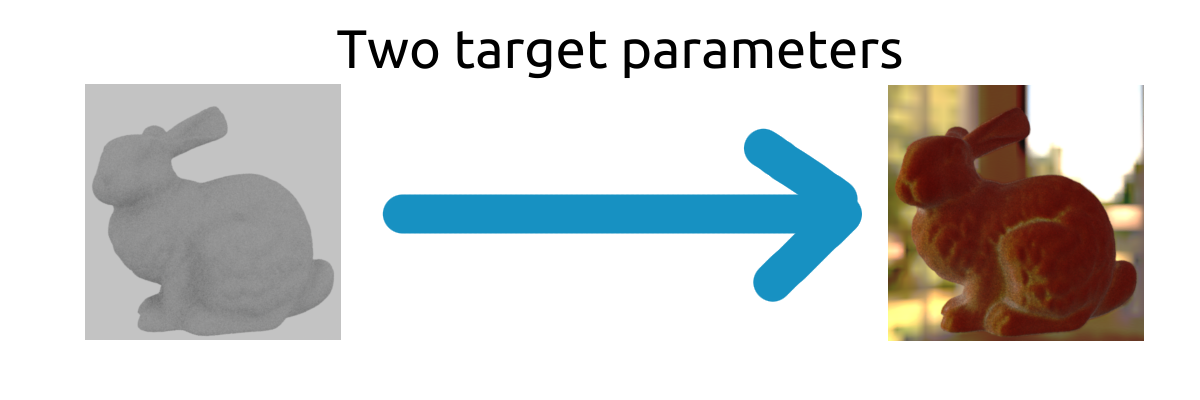
\includegraphics{./figures/Intro-1.png}
        \end{figure}
    \end{itemize}
\end{frame}
\end{document}